%%MAIN: thesis.tex

%%%%% Background Information %%%%%
\chapter{Technical Background} \label{ch_background}

The product of this thesis is implemented in Glamorous Toolkit and bases teaching material on the ``Processing'' programming language. A brief overview of both is given in this chapter for readers unaware of either of them.



\section{Processing} \label{sc_processing}

``Processing'' is a programming language consisting of a graphics API built upon a mainstream language as a base. Development started between 1997 and 2004 at the MIT Media Lab with the goal of creating a language for teaching art students the fundamentals of programming as basis for creating digital, visual art.

Its authors, Reas and Fry \cite{Rea14}, wanted to create a unified teaching system consisting of art, language and a matching IDE. They based the language upon then popular and portable Java, removing much of the boilerplate required for object orientation, enhancing it with visual primitives and implicitly showing an output window, allowing for quick results (see figure \ref{fig_alpinerWanderweg}).

\begin{figure} \label{fig_alpinerWanderweg}
\begin{minipage}{.5\textwidth}
\begin{code}
// Output canvas dimensions
size(200, 200);
// (Default white) square
rect(50, 50, 100, 100);
// Red inner rectangle
fill(255, 0, 0);
rect(50, 50 + 100 / 3, 100, 100 / 3);
\end{code}
\end{minipage}
\begin{minipage}{.45\textwidth}
\centering

\includegraphics[height=3cm]{images/alpinerWanderweg}
\end{minipage}
\lessSpace
\caption{Example code (with Java syntax) and output}
\end{figure}

As elaborated in \ref{ssc_top_down}, Processing was meant to be taught top down, starting from art and then decomposing it. As such, its main introduction features several chapters focused on exhibits of digital or hybrid art such as Manfred Mohr's \emph{Une esth�tique programm�e} or Steph Thirion's \emph{Eliss}.

Apart from graphical primitives (see appendix \ref{app_api} for the API subset implemented for this thesis), Processing features an implicit event loop which allows for creating (interactive) animations within a dozen lines of code (see figure \ref{fig_jumpingBall}).

\begin{figure} \label{fig_jumpingBall}
\begin{minipage}{.5\textwidth}
\begin{code}
y = 50; dy = 0

# called once after global code
def setup():
    size(100, 200)

# called repeatedly for every frame
def draw():
    global y, dy
    background(192)
    circle(50, y, 50)
    y += dy; dy += 1
    if y > height - 25:
        dy = -0.9 * dy
\end{code}
\end{minipage}
\begin{minipage}{.45\textwidth}
\centering

\includegraphics[height=3cm]{images/ball1}

\includegraphics[height=3cm]{images/ball2}

\includegraphics[height=3cm]{images/ball3}

\includegraphics[height=3cm]{images/ball4}
\end{minipage}
\lessSpace
\caption{Example code (with Python syntax) and one output frames}
\end{figure}

Reacting to input happens either by pulling state while painting a frame (implicit global variables \ct{mousePressed}, \emph{etc.}) or by defining event handlers alongside \ct{setup} and \ct{draw}.

Since Python has become the prevalent teaching language (\cite{Cod20}), Processing has been extended with a Python mode which leads to Processing code reading like Python code with the additional Processing API calls and exposes most of Python's libraries to Processing code. This allows using Processing as a starting language and later seamlessly transitioning to pure Python code, which remains part of the motivation for students: learning an ``actually useful'' language.

As the official Processing IDE continues to be written in Java, Processing's official Python mode uses Jython for compiling the code to Java Bytecode. Since developers have started moving away from Java, there are now several reimplementations of Processing such as p5.js for running Processing on top of JavaScript in a web environment, p5.py for running Processing in a pure Python environment\footnote{Requiring two additional lines: \ct{from p5 import *} at the top and \ct{run()} at the bottom.} or a version of Processing for microcontrollers such as Arduino. With this thesis, a limited version for a Smalltalk environment is also available.

Initially in the early 2010s, we ran our own IDE based on p5.js with custom error handling\footnote{This is still available from \url{https://software.zeniko.ch/ProcessingIDE.zip}. Note that it's targeted at \ct{mshta.exe} and as such runs best under Windows.} before changing to the official IDE for its Python mode.

Our experience of working with Processing over the past decade has shown that it allows novice programmers in the first year of high school to learn enough of the language within a month that they're able to write a clone of a game like ``Pong'', ``Flappy Bird'' or ``Geometry Dash'' as a group project. Feedback from the various student groups about this part of the computer science curriculum has always been positive to very positive. This aligns with what didactics states about student motivation (see \ref{sc_didactic}).



\section{Moldable Development} \label{sc_moldable}

``Moldable development'' is a term coined by Nierstrasz and G�rba \cite{Gir22,Nie24} for a collection of development patterns which should make it easier to understand a computer system by extending (`molding') it with views and features. The goal of moldable development is to quickly get feedback on code and objects being worked on so that a programmer can confidently make appropriate changes.

In traditional IDEs, a running system is inspected either through its source code or its live runtime objects. Available views (see \ref{ssc_ides}) are static and new views are added through non-trivial extensions. Moldable development asks for an environment in which a tool is more easily adaptable to data, making it simple to write either one-off throw-away views and tools but also allowing to refactor such throw-away code into reusable components when needed.

Moldable development is thus a form of exploratory programming (cf. \ref{ssc_exploration}) on live objects where tools, whether one-off or reusable, are created in a bottom up approach with immediate feedback available at every step.

In order to support this, a moldable environment must have extensibility in its core, allowing to register tools and views e.\,g. through a simple code annotation of a few characters which the environment can use to detect and include it (instead of having to write a lot of configuration boilerplate and overhead which IDE extensions meant for independent distribution usually involve).

One core pattern of moldable development is the ``Moldable Object'': Objects should be implementable incrementally with live object states and previously developed views remaining available throughout the whole process. An object consisting of little more than a data wrapper is thus extended with new functionality as it fits the available live data -- instead of designing an object on a clean slate or along tests. Exploration code can then be extracted into tests, ensuring that what worked once will continue to work. Extending objects iteratively based on actual needs ensures that they remain transparent and that code is cleanly separated.

Having a moldable environment also allows for working on code and documentation intertwined, similar to literate programming \cite{Knu84}. Opposed to literate programming where code has to be extracted first, in moldable development every code snippet should be runnable on its own and beside code and documentation also live results can be included. This allows a moldable environment to be used to either first document ideas and then add matching code but also to document progress or explain written code (which can then easily be extracted into a test case).

For students, such a ``Project Diary'' pattern could be used as a learning journal (similar to Microsoft OneNote), for project exploration (similar to Jupyter notebooks) or for project documentation. Another useful pattern for teaching is the ``Composed Narrative'' which visualizes object relations through side-by-side views tailored towards explaining a relation or interaction.



\section{Glamorous Toolkit} \label{sc_gt}

``Glamorous Toolkit'' (GT) is a fully programmable environment optimized for moldable development (see \ref{sc_moldable}). It is programmed in Smalltalk and by default persists its entire state into an \ct{.image} file when shut down so that live objects don't have to be recreated at restart \cite{Gir23}.

Smalltalk environments have had that property since the early days in the 1970s, when Alan Kay sketched out the original Smalltalk which he eventually standardized at Xerox into Smalltalk-80. Based on a Smalltalk-80 virtual machine by Apple, Ingals, Kay \emph{et al.} started developing a new virtual machine and development environment, Squeak, which had the goal to also be customizable by non-programmers \cite{Ing97}. Squeak inherited its built-in capabilites for live and exploratory coding from the original Smalltalk and its back to this point that GT's heritage is tied directly.

While Squeak was further developed at Walt Disney Media Labs and among others included in the ``One Laptop per Child'' laptops, it remained a niche product -- likely due to missing interoperability between the live environment inside its virtual machine and outside code. Still, Squeak and its later fork Pharo continued being worked on and were actively being used in academia and related spin-offs. Eventually, a team around Tudor G�rba -- including this thesis' supporter Oscar Nierstrasz -- set out to implement their idea of a moldable environment on the basis of Pharo, thus creating Glamorous Toolkit \cite{Fee25}. Version 1.0 has been released in 2023 and is still being actively worked on.

Glamorous Toolkit thus has an illustrious lineage and has achieved support for many concepts asked for by literature (as outlined in \ref{sc_didactic} and \ref{sc_moldable}): It's a moldable environment, supports a clean object-oriented language, allows for live and exploratory programming, still remains comparatively manageable and -- particularly relevant for this thesis -- allows for reflection at various levels, including for every object access to its method's source code, its compiled form and even its memory layout inside the virtual machine.

GT provides a tabbed interface which can show one of several tools: an object viewer, a notebook (dubbed ``Lepiter''), a code browser, a git interface and many more. While such tools are about as difficult to implement as an IDE extension, the object viewer -- a tabbed interface itself -- is extended by annotating an object method which returns a \ct{GtPhlowView} object with \ct{<gtView>}:

\begin{code}
ProcessingCodeBase >> gtOutputFor: aView [
	<gtView>
	^ aView explicit
		title: 'Output' translated;
		priority: 40;
		stencil: [ (ProcessingRunner new
				limitTo: (self gtIsAnimation ifTrue: [ 30 ] ifFalse: [ 2 ]) seconds;
				run: self clone;
				canvas) asElement ]
]
\end{code}

\begin{figure} \label{fig_gt_screenshot}
\centering
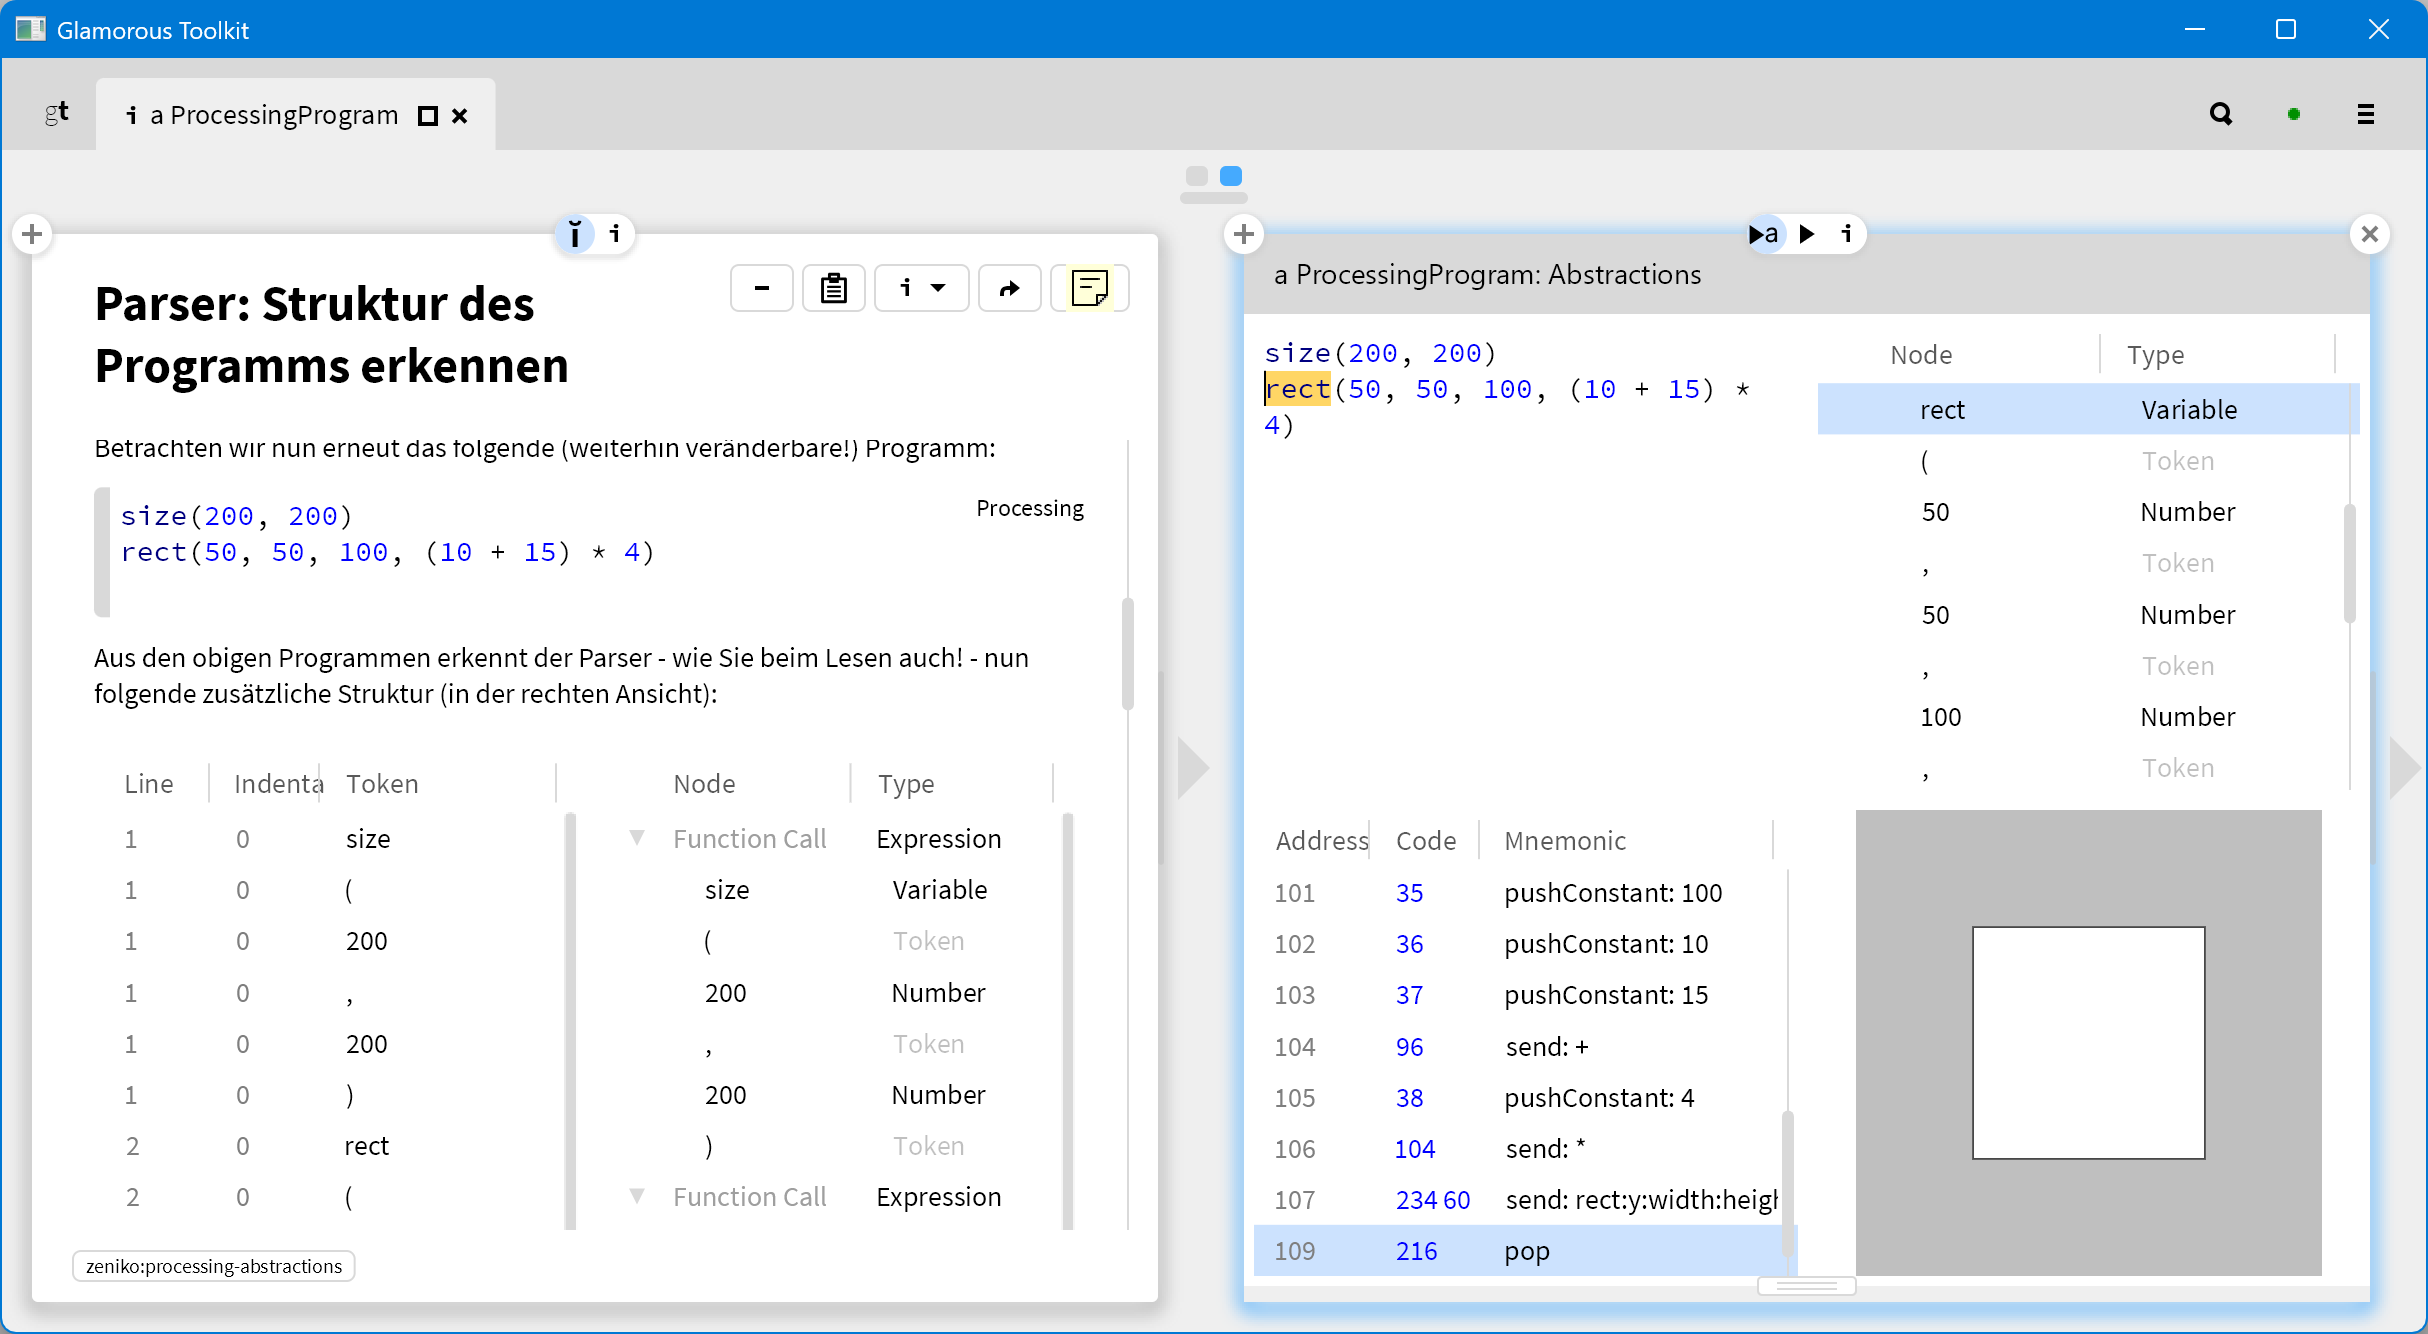
\includegraphics[height=3cm]{images/gt_screenshot}
\lessSpace
\caption{GT with a live notebook page (left) and inspectable object view (right)}
\end{figure}

The element passed to the \ct{stencil:} message -- here the canvas resulting from running a Processing program -- could instead also be displayed inside a notebook page, with no annotations needed at all.

Annotations are thus only required to allow GT to discover messages of a certain type. Similarly, methods annotated with \ct{<gtExample>} are considered tests and can be collectively inspected and run for a class or an entire package. This achieves several goals of moldable development: What starts as throw-away code can be extracted into a method, annotated and remains then permanently available for repeated testing. Examples are also includable by name in notebooks, where they do function as (tested and thus guaranteed working) examples for documentation.

While GT is based on a Smalltalk virtual machine, support for other modern languages such as Python, JavaScript or Java has been added through a language bridge connecting to an external virtual machine and allowing for inspection and visualization of objects originating there. Unfortunately, these language bridges are one example where one of GT's drawbacks starts showing.

\subsection{Bleeding Edge}

GT follows a trunk-only development style without release branches. This means that downloading GT on two different days might result in subtle differences. If GT with an app is to be distributed, the best way to do this is by downloading the latest version, loading the app into it, testing it and then distributing \emph{this known good} image (as is described in \ref{app_setup}). Also, GT is mainly developed under macOS and makes some platform assumptions with relation to its host operating system. This isn't noteable when working purely within GT but occasionally shows at its seams.

What might also take some getting used to: All the code in GT and all live objects are stored in its \ct{.image} file and are updated whenever GT is closed with saving. Synchronization of Smalltalk code thus happens best through GT's built-in git client. Preexisting notebook pages are also stored within one of GT's subdirectories. Users can however create new pages in the ``Local knowledge base''\footnote{By default, this is located in the \ct{lepiter} subdirectory of the user's documents or home folder.} which can be backed up separatedly and which are stored even when GT is quit without saving. All notebook pages indicate where they're stored in their footer and can be moved between databases through that footer. This allows students to take an existing page from teaching material and move it locally where it's separately backed up, in case they later delete or update GT.
